% Drawing 69/06-6 -- folder 69, batch 06, archive page 112 (PDF page 113).
% Transcription: à gauche, un premier triangle très surchargé, aux sommets $P_1$, $P_2$, $P_3$ et aux côtés marqués $G_1$, $G_2$, $G_3$, $G'_3$, dont les indices sont repassés, raturé de plusieurs traits ; à droite, le triangle mis au net : $P_1$ en haut, $P_3$ en bas à gauche, $P_2$ en bas à droite, les côtés marqués $G_2$ (entre $P_1$ et $P_3$), $G_3$ (entre $P_1$ et $P_2$), $G_1$ (entre $P_3$ et $P_2$)
% Kind: overwritten triangle and its fair copy. Method 2 (schematic redraw from the facsimile). Status: ok.
% Notes: Left: a first triangle, heavily overwritten and struck (drawn grey), vertices P_1, P_2, P_3, sides G_1, G_2, G_3, G'_3. Right: the fair copy, P_1 at the top, P_3 lower left, P_2 lower right, sides G_2 (P_1 P_3), G_3 (P_1 P_2), G_1 (P_3 P_2).
% Coordinates: 1 unit = 1 mm = 1/100 of the crop width (bbox in page fractions: [0.08, 0.05, 0.5, 0.17]).
% Redrawn by Claude (claude-opus-5-5), issue #73, 2026-11-07; not checked by a human; not compiled (no TeX in the session).
% Rights: reproduces part of the work -- behind RENDER_TRANSCRIPTS, never published by itself.
\documentclass[tikz,border=3pt]{standalone}
\usepackage{amsmath,amssymb}
\usetikzlibrary{patterns,arrows.meta}
\tikzset{pencil/.style={black!45}, struck/.style={black!35}, mark/.style={circle,draw,inner sep=1.3pt}, pt/.style={circle,fill,inner sep=0.9pt}, opt/.style={circle,draw,fill=white,inner sep=1.1pt}}
\begin{document}
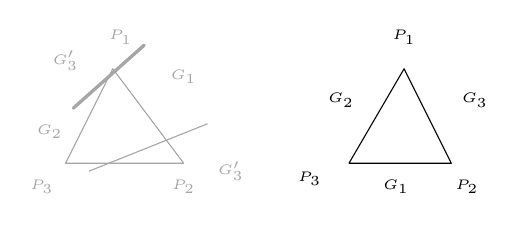
\begin{tikzpicture}[x=1mm,y=1mm,line cap=round,line join=round,font=\scriptsize]
\draw[struck] (36,-19) -- (30,-31) -- (45,-31) -- cycle;
\draw[struck,very thick] (31,-24) -- (40,-16);
\draw[struck] (33,-32) -- (48,-26);
\node[inner sep=1pt,struck] at (37,-15) {\tiny $P_1$};
\node[inner sep=1pt,struck] at (30,-18) {\tiny $G'_3$};
\node[inner sep=1pt,struck] at (45,-20) {\tiny $G_1$};
\node[inner sep=1pt,struck] at (28,-27) {\tiny $G_2$};
\node[inner sep=1pt,struck] at (27,-34) {\tiny $P_3$};
\node[inner sep=1pt,struck] at (45,-34) {\tiny $P_2$};
\node[inner sep=1pt,struck] at (51,-32) {\tiny $G'_3$};
\draw (73,-19) -- (66,-31) -- (79,-31) -- cycle;
\node[inner sep=1pt] at (73,-15) {\tiny $P_1$};
\node[inner sep=1pt] at (61,-33) {\tiny $P_3$};
\node[inner sep=1pt] at (81,-34) {\tiny $P_2$};
\node[inner sep=1pt] at (65,-23) {\tiny $G_2$};
\node[inner sep=1pt] at (82,-23) {\tiny $G_3$};
\node[inner sep=1pt] at (72,-34) {\tiny $G_1$};
\end{tikzpicture}
\end{document}
